% IEEEtran port of the manuscript (generated 2026-08-15).
% For IEEE Access, switch to the official Access template (ieeeaccess.cls) and
% paste the section bodies across; the structure below maps one-to-one.
%
% Remaining author action before submission:
%  - Re-check ref [21] (medRxiv preprint) for a peer-reviewed version.
% Table VI rows were all verified against primary sources on 2026-08-15.
\documentclass[journal]{IEEEtran}

\usepackage[T1]{fontenc}
\usepackage[utf8]{inputenc}
\usepackage{graphicx}
\usepackage{amsmath}
\usepackage{booktabs}
\usepackage{textcomp}
\usepackage{url}

\begin{document}

\title{Tuberculosis Is Not in the Corner of the Image: A Cross-Dataset Study of
Shortcut Learning and the Limits of Lung Segmentation in Chest-Radiograph
Classifiers}

\author{Alvin~Chow%
\thanks{A. Chow is an independent researcher (e-mail: alvinchow97@gmail.com).}}

\maketitle

\begin{abstract}
Deep learning achieves near-perfect tuberculosis (TB) detection on chest
radiographs within a single dataset, but such figures are rarely validated
across institutions. We train a MobileNetV2 classifier on a public TB
radiography database and evaluate it, under a leakage-safe protocol with
bootstrap confidence intervals, on two independent National Library of Medicine
cohorts (Montgomery and Shenzhen). In-domain area under the ROC curve (AUC)
reaches 0.9995 but falls to 0.70--0.78 externally --- an approximately 0.25 AUC
generalisation gap whose confidence intervals do not overlap the in-domain
estimate, and which five-fold cross-validation confirms is stable
($0.25 \pm 0.02$ AUC). We show that the accompanying collapse of sensitivity to
near zero is largely a threshold-transfer artefact: the optimal operating point
shifts roughly fivefold between sources, while the underlying discrimination
ceiling is about 70\,\% sensitivity at 70\,\% specificity. A duplicate-image
audit confirms the external cohorts share no overlap with the training data, so
the gap is a genuine out-of-source failure. We then test the two most commonly
recommended mitigations. Intensity harmonisation combined with augmentation and
multi-source training improves external AUC only marginally ($+0.02$). Lung
segmentation, using a U-Net segmenter of high quality (Dice 0.975) producing
anatomically sound masks, fails to close the gap and in fact degrades unbiased
external AUC in every cross-validation fold (paired decrease $0.057 \pm 0.011$;
0.776 to 0.662 on the primary split) --- contrary to prior reports for COVID-19
radiography. The failure is moreover architecture-dependent: identically
trained DenseNet-121 and EfficientNet-B0 backbones match MobileNetV2 in-domain
(all $\geq 0.999$) yet each collapses on a \emph{different} external cohort
(DenseNet to chance on Shenzhen, $0.503 \pm 0.025$; EfficientNet to
near-chance on Montgomery, $0.541 \pm 0.061$), so the two cohorts rank the
three architectures in entirely different orders, and a frozen-feature probe
shows this divergence already exists in the pretrained representations before
any fine-tuning. Segmentation interacts with this dependence in a structured
way: masking significantly degrades the best raw transfer while significantly
recovering the collapsed ones, homogenising all three backbones into a common
0.61--0.77 band well below in-domain performance. We conclude that the TB-CXR
generalisation gap is real, large, and resistant to the standard playbook; that
single-cohort external validation can invert architecture rankings; and that
out-of-source external validation on multiple cohorts must be treated as
mandatory rather than optional.
\end{abstract}

\begin{IEEEkeywords}
Tuberculosis, chest radiography, deep learning, shortcut learning, domain
generalisation, lung segmentation, external validation, model calibration.
\end{IEEEkeywords}

\section{Introduction}

\IEEEPARstart{T}{uberculosis} remains among the leading causes of death from
infectious disease worldwide, and the chest radiograph (CXR) is a primary
screening modality, particularly where expert readers are scarce. Convolutional
neural networks have reported radiologist-level performance on CXR
tasks~\cite{rajpurkar2017chexnet} and TB-specific AUCs as high as
0.99~\cite{lakhani2017deep}, motivating interest in automated TB screening.

Such headline figures, however, are usually obtained and reported on a single
data source. Recent work shows that high in-distribution accuracy can reflect
\emph{shortcut learning}~\cite{geirhos2020shortcut}, in which a model exploits
dataset-specific cues that fail under distribution shift. In radiography this
is documented: a pneumonia classifier learned to detect a hospital-specific
metal token~\cite{zech2018variable}, and COVID-19 classifiers were shown to
rely on confounders rather than pathology~\cite{degrave2021ai}. Cross-dataset
performance drops have also been reported for TB classifiers trained on
single-hospital data~\cite{sathitratanacheewin2020deep, karki2022generalization,
shuaibu2026geographic}. However, for the multi-source composite database that
has become the most widely used TB-CXR training benchmark --- whose Normal and
TB images are drawn from different source archives, an almost ideal setting for
shortcut learning --- the magnitude of the gap, its decomposition, and above
all whether the standard mitigations close it, remain unexamined.

This paper makes the following contributions. (1)~We quantify the in-domain
versus external generalisation gap for a standard TB-CXR classifier with
bootstrap confidence intervals under a leakage-safe evaluation protocol, and
confirm its stability with five-fold cross-validation and a duplicate-image
audit. (2)~We decompose the external failure into a threshold-transfer
component and a discrimination component. (3)~We evaluate the two
most-recommended mitigations --- intensity harmonisation with augmentation and
multi-source training, and lung segmentation --- and find that neither closes
the gap; segmentation, despite a high-quality segmenter, \emph{degrades}
unbiased external performance in every cross-validation fold, contradicting
prior COVID-CXR findings~\cite{bassi2022covid}. (4)~We show the failure is
architecture-dependent --- DenseNet-121 and EfficientNet-B0 with identical
training match in-domain performance but each collapses on a \emph{different}
external cohort, inverting the architecture ranking between cohorts --- and,
with a frozen-feature probe, that each profile is inherited from the pretrained
representations rather than induced by fine-tuning; we further show that
masking homogenises all three backbones into a common sub-clinical band,
degrading the best transfer while recovering the collapsed ones. (5)~We draw
the practical conclusion that out-of-source external validation on more than
one cohort is a prerequisite for trusting a TB-CXR model, and that neither
segmentation nor any single backbone should be assumed to confer robustness.

\begin{figure*}[!t]
\centering
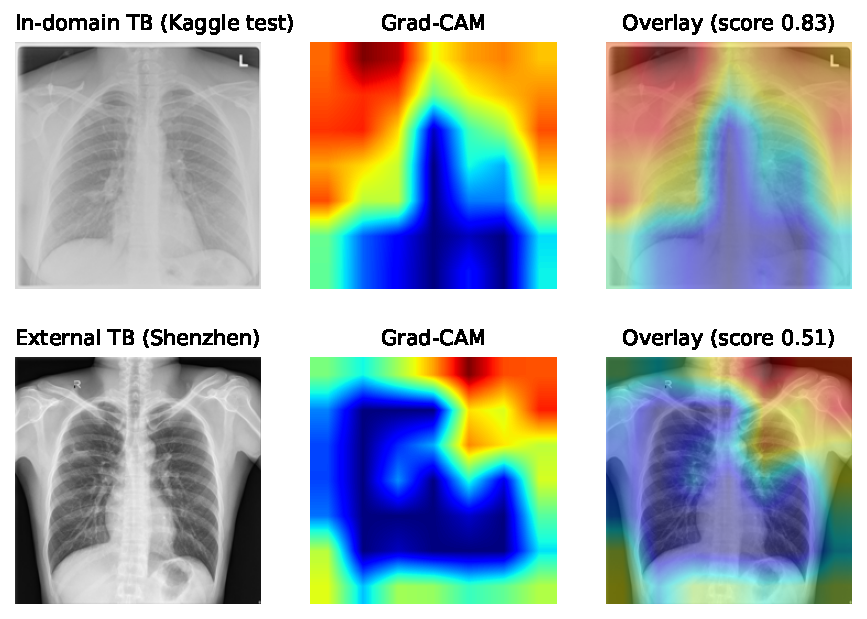
\includegraphics[width=0.85\textwidth]{figures/fig1_gradcam.pdf}
\caption{Grad-CAM attention for the baseline model. Top row: an in-domain TB
case (score 0.83, detected). Bottom row: a median-scoring external TB case
(Shenzhen; score 0.51, below the 0.648 operating threshold and therefore
missed). In both, attention falls largely on image borders and the mediastinum
rather than inside the lung fields --- qualitative evidence of shortcut
reliance.}
\label{fig:gradcam}
\end{figure*}

\section{Related Work}

\subsection{Deep Learning for Chest Radiography}
Rajpurkar \emph{et al.}~\cite{rajpurkar2017chexnet} trained a 121-layer
DenseNet on over 100\,000 images and reported pneumonia detection exceeding
radiologist performance on a held-out set. For tuberculosis, Lakhani and
Sundaram~\cite{lakhani2017deep} obtained an AUC of 0.99 with
ImageNet-pretrained CNNs. The systematic review of Hansun
\emph{et al.}~\cite{hansun2023machine}, covering 47 studies, documents rapid
growth alongside recurring methodological weaknesses, notably limited external
validation.

\subsection{Shortcut Learning and Generalisation}
Geirhos \emph{et al.}~\cite{geirhos2020shortcut} frame shortcut learning as
decision rules that succeed on benchmarks but fail out-of-distribution, with
out-of-distribution testing as the diagnostic. Zech
\emph{et al.}~\cite{zech2018variable} found significant cross-hospital
degradation for pneumonia and identified a non-pathological confounder; DeGrave
\emph{et al.}~\cite{degrave2021ai} showed COVID-19 classifiers relied on
confounders and argued explainability is a deployment prerequisite.

\subsection{Cross-Dataset TB Validation}
Sathitratanacheewin \emph{et al.}~\cite{sathitratanacheewin2020deep} trained on
the Shenzhen set and observed AUC fall from 0.85 (intramural) to 0.71 on NIH
ChestX-ray8. Karki \emph{et al.}~\cite{karki2022generalization} reported a
comparable drop for drug-resistant TB and found that multi-task training with
lesion-location supervision partially recovered external performance. A recent
multi-national study~\cite{shuaibu2026geographic} describes geographically
divergent failure modes for a Shenzhen-trained DenseNet-121 (false-positive
surge in a low-burden cohort, sensitivity collapse in a high-burden one). All
of these train on a single source archive and evaluate one architecture; none
quantifies the gap for the multi-source Kaggle composite, tests lung
segmentation as a mitigation, or examines whether the failure is
architecture-dependent --- the three axes of the present study.

\subsection{Mitigations}
Lung segmentation is the most advocated remedy, removing out-of-lung pixels:
Bassi and Attux~\cite{bassi2022covid} reported it improved external COVID-19
performance, Teixeira \emph{et al.}~\cite{teixeira2021impact} likewise found it
important for COVID-19 generalisation, and it has been used (with histogram
equalisation and rib suppression) to debias lung-nodule datasets --- typically
via a U-Net~\cite{ronneberger2015unet}. To our knowledge its effect on
\emph{cross-dataset TB} generalisation has not been tested. Harmonisation
(e.g.\ contrast-limited adaptive histogram equalisation) and augmentation
target intensity cues. We evaluate both directly.

\subsection{Evaluation Rigour}
Rouzrokh \emph{et al.}~\cite{rouzrokh2022mitigating} identify image-level
(versus patient-level) splitting as a primary source of optimistic bias, and
Tampu \emph{et al.}~\cite{tampu2022inflation} quantify inflation up to
${\sim}0.43$ in Matthews correlation coefficient. These inform our
interpretation of high in-domain figures and our stated limitations.

\section{Materials and Methods}

\subsection{Datasets}
The in-domain data is the public TB Chest Radiography Database (3\,500 Normal,
700 TB), split 80/10/10 with stratification. External validation uses two NLM
cohorts~\cite{jaeger2014two}: Montgomery County (80 Normal, 58 TB) and Shenzhen
Hospital (326 Normal, 336 TB). Montgomery distributes ground-truth lung masks,
used to train the segmenter. Source heterogeneity between archives is the
suspected origin of the confound.

\subsection{Model and Training}
A MobileNetV2 backbone~\cite{sandler2018mobilenetv2} pretrained on ImageNet is
used with global average pooling, dropout, and a sigmoid output. Images are
preprocessed with the MobileNetV2 transform to $[-1, 1]$. Training is two-stage
transfer learning (frozen-backbone head training, then fine-tuning) with focal
loss~\cite{lin2017focal} to address the 5:1 class imbalance; gradient clipping
(clipnorm $= 1.0$) is applied for training stability.

\subsection{Evaluation Protocol}
To avoid leakage, the operating threshold is selected on the validation set at
sensitivity $\geq 0.90$ and applied once to each test set. We report ROC-AUC
and PR-AUC with 2\,000-resample bootstrap 95\,\% confidence intervals, plus
sensitivity and specificity. Calibration is measured by expected calibration
error (ECE) with temperature scaling~\cite{guo2017calibration} fitted on the
validation set. Grad-CAM~\cite{selvaraju2017gradcam} and Integrated
Gradients~\cite{sundararajan2017axiomatic} provide attention visualisations.
Robustness is assessed by five-fold stratified cross-validation, and data
integrity by a duplicate-image audit (exact MD5 plus a 256-bit difference
hash).

\subsection{Mitigation A}
CLAHE intensity harmonisation, stronger augmentation (rotation, zoom,
translation, contrast), reduced fine-tuning depth with increased dropout, and
multi-source training under a leave-one-dataset-out design (train on Kaggle
$+$ Shenzhen, hold out Montgomery).

\subsection{Mitigation B}
A U-Net~\cite{ronneberger2015unet} lung segmenter is trained on the 138
Montgomery mask pairs with a combined BCE--Dice loss. The trained segmenter
masks all cohorts; a classifier identical to the baseline except for masked
input is trained on masked data. Shenzhen, unseen by the segmenter, is the
unbiased external test.

\subsection{Backbone Study and Frozen-Feature Probe}
To test whether the findings are specific to MobileNetV2, the five-fold
cross-validation is repeated with DenseNet-121 and EfficientNet-B0 backbones
under an identical protocol --- the same fold assignments, head architecture,
two-stage training schedule, and focal loss --- with each backbone paired with
its own canonical input preprocessing, in both raw and masked-input conditions.
To localise the origin of any backbone-dependent behaviour, we additionally run
a frozen-feature probe: ImageNet-pretrained features are extracted from each
backbone's global-average-pooled output \emph{without any fine-tuning}, and an
L2-regularised logistic regression is fitted on the training-split features and
evaluated on the in-domain test split and both external cohorts. Because the
probe involves no gradient updates to the backbone, any external failure it
reproduces must be a property of the pretrained representation interacting with
the dataset shift, not of the training procedure. As a low-level check, we also
measure the discriminative power of mean image brightness alone per cohort, and
the Spearman correlation between each probe's scores and image brightness.

\section{Results}

\subsection{Generalisation Gap}
In-domain test AUC was 0.9995 (95\,\% CI 0.998--1.000; PR-AUC 0.998), falling
to 0.776 (0.740--0.811) on Shenzhen, 0.698 (0.607--0.784) on Montgomery, and
0.752 (0.719--0.786) pooled (Table~\ref{tab:gap}). Confidence intervals for the
external cohorts do not overlap the in-domain estimate; an unpaired bootstrap
difference confirms the in-domain--Shenzhen gap is significant
($\Delta = 0.22$, 95\,\% CI 0.19--0.26, $p < 0.001$). The corresponding ROC
curves are shown in Fig.~\ref{fig:roc}.

\begin{table}[!t]
\caption{In-Domain vs External Discrimination (95\,\% Bootstrap CIs)}
\label{tab:gap}
\centering
\begin{tabular}{lccc}
\toprule
Evaluation & ROC-AUC (95\,\% CI) & Sens. & Spec. \\
\midrule
In-domain (Kaggle) & 0.9995 (0.998--1.000) & 0.93 & 1.00 \\
Shenzhen & 0.776 (0.740--0.811) & 0.02 & 1.00 \\
Montgomery & 0.698 (0.607--0.784) & 0.00 & 1.00 \\
Combined & 0.752 (0.719--0.786) & 0.02 & 1.00 \\
\bottomrule
\end{tabular}
\end{table}

\begin{figure}[!t]
\centering
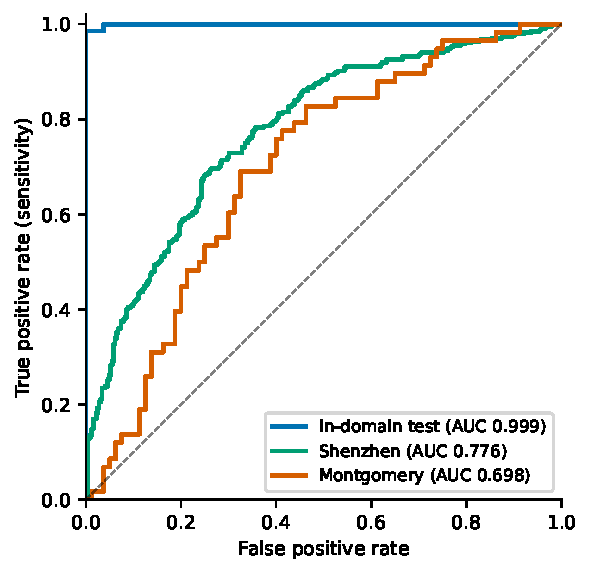
\includegraphics[width=\columnwidth]{figures/fig2_roc.pdf}
\caption{ROC curves for the baseline classifier: in-domain test (AUC 0.9995)
versus Montgomery (0.698) and Shenzhen (0.776), illustrating the
${\sim}0.25$ AUC generalisation gap.}
\label{fig:roc}
\end{figure}

\subsection{Threshold vs Discrimination}
At the in-domain threshold (0.648) external sensitivity was ${\approx}0$; the
model required thresholds of 0.05--0.23 externally. At a balanced (Youden)
operating point the cohorts reached ${\approx}0.71/0.69$ (combined)
sensitivity/specificity (Table~\ref{tab:threshold}), indicating the collapse is
partly threshold-transfer and partly a discrimination ceiling.

\begin{table}[!t]
\caption{External Performance by Operating Point}
\label{tab:threshold}
\centering
\begin{tabular}{lccc}
\toprule
Cohort & AUC & thr 0.648 (se/sp) & Youden (se/sp) \\
\midrule
Montgomery & 0.698 & 0.00 / 1.00 & 0.83 / 0.54 \\
Shenzhen & 0.776 & 0.02 / 1.00 & 0.68 / 0.75 \\
Combined & 0.752 & 0.02 / 1.00 & 0.71 / 0.69 \\
\bottomrule
\end{tabular}
\end{table}

\subsection{Calibration}
ECE was 0.770 before and 0.833 after temperature scaling (fitted $T = 0.12$);
the perfectly separated validation set makes the fit degenerate, so calibration
could not be corrected (Fig.~\ref{fig:reliability}).

\begin{figure*}[!t]
\centering
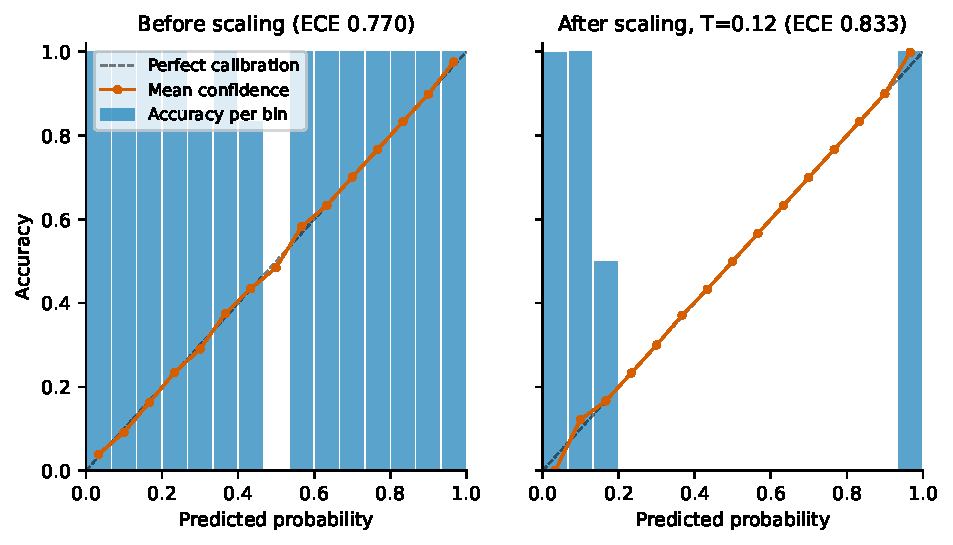
\includegraphics[width=0.85\textwidth]{figures/fig3_reliability.pdf}
\caption{Reliability diagrams on the in-domain test set, before (ECE 0.770) and
after (ECE 0.833) temperature scaling, showing that scaling fails to correct
the over-confident, saturated probabilities.}
\label{fig:reliability}
\end{figure*}

\subsection{Mitigation A}
External (Montgomery) AUC improved from 0.698 to 0.719 ($+0.021$) while
in-domain fell from 0.999 to 0.966 (Table~\ref{tab:mitigations}); the gap
narrowed chiefly through reduced over-fitting.

\subsection{Mitigation B}
The segmenter achieved validation Dice 0.975; retained lung-pixel fractions
were 0.26--0.31 across all cohorts (Shenzhen 0.29) with no degenerate masks
(Fig.~\ref{fig:segmentation}). On the primary split, masked-input AUC was 0.998
in-domain, 0.728 on Montgomery (confounded; segmenter trained on Montgomery),
and 0.662 on Shenzhen --- a decrease of 0.114 versus the raw baseline on the
unbiased cohort (Table~\ref{tab:mitigations}), significant by DeLong's test for
correlated ROC curves ($z = 4.65$, $p < 0.001$). The cross-validated,
fold-paired comparison confirms the direction while tempering the magnitude:
masking reduced Shenzhen AUC in \textbf{all five folds} (raw $0.743 \pm 0.030$
vs masked $0.686 \pm 0.030$; paired decrease $0.057 \pm 0.011$, paired
$t = 11.9$, $p < 0.001$), whereas the Montgomery difference was not consistent
across folds (mean $-0.009$, mixed signs). We therefore report the
cross-validated paired decrease of ${\approx}0.06$ AUC as the primary estimate
of the segmentation penalty, with the single-split value of 0.114 as one
realisation. Section~\ref{sec:backbones} shows this penalty is specific to the
MobileNetV2 backbone: for architectures whose raw external transfer had
collapsed, the same masking instead \emph{recovers} performance --- into the
same mediocre band.

\begin{table}[!t]
\caption{Mitigation Results (AUC)}
\label{tab:mitigations}
\centering
\begin{tabular}{lccc}
\toprule
Condition & In-domain & Montgomery & Shenzhen$^{*}$ \\
\midrule
Baseline (raw) & 0.999 & 0.698 & 0.776 \\
Mitigation A & 0.966 & 0.719 & --- \\
Mitigation B (masked) & 0.998 & 0.728 & 0.662 \\
\bottomrule
\multicolumn{4}{l}{\footnotesize $^{*}$Shenzhen is the unbiased external
cohort (unseen by the segmenter).}
\end{tabular}
\end{table}

\begin{figure*}[!t]
\centering
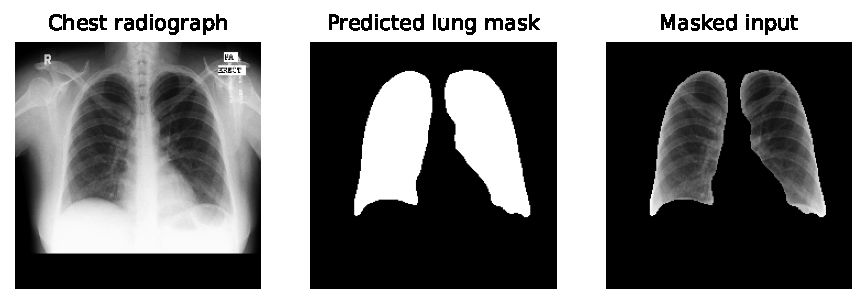
\includegraphics[width=0.85\textwidth]{figures/fig4_segmentation.pdf}
\caption{Lung segmentation example: original chest radiograph, U-Net predicted
lung mask, and the resulting masked input fed to the classifier (Dice 0.975 on
held-out Montgomery masks).}
\label{fig:segmentation}
\end{figure*}

\subsection{Robustness: Five-Fold Cross-Validation}
To confirm the gap is not an artefact of a single split, we ran five-fold
stratified cross-validation on the Kaggle data, evaluating each fold's model on
the fixed external cohorts (Table~\ref{tab:cv}). The gap is stable: in-domain
AUC $0.9991 \pm 0.0009$, Montgomery $0.6884 \pm 0.0040$, Shenzhen
$0.7461 \pm 0.0215$, giving a generalisation gap (in-domain minus Shenzhen) of
$0.2530 \pm 0.0223$. The small per-fold variance --- Montgomery ranged only
0.682--0.694 --- indicates the gap is a stable property of the source mismatch
rather than of any particular split.

\begin{table}[!t]
\caption{Five-Fold Cross-Validation (AUC, Mean $\pm$ Std)}
\label{tab:cv}
\centering
\begin{tabular}{lc}
\toprule
Evaluation & AUC (mean $\pm$ std) \\
\midrule
In-domain & $0.9991 \pm 0.0009$ \\
Montgomery & $0.6884 \pm 0.0040$ \\
Shenzhen & $0.7461 \pm 0.0215$ \\
Gap (in-domain $-$ Shenzhen) & $0.2530 \pm 0.0223$ \\
\bottomrule
\end{tabular}
\end{table}

\subsection{Data-Overlap Audit}
Because the in-domain AUC is near-perfect, we audited for duplicate leakage
using exact MD5 hashing and a discriminative 256-bit difference hash (a coarse
hash over-reports duplicates for radiographs, which share gross structure).
Within Kaggle, only two byte-identical files and a small number of
near-duplicate pairs (Hamming $\leq 10$, all within-class) span the train/test
boundary, affecting ${\approx}1\,\%$ of the test set --- far too few to account
for the in-domain AUC, which instead reflects genuine within-source
separability. The cross-cohort check deserves particular care because the
composite database's own documentation lists the NLM Montgomery and Shenzhen
collections among its candidate sources~\cite{rahman2020reliable}: if the
public release actually contained those images, our ``external'' cohorts would
not be external at all. Three independent checks refute this for the public
release used here. No exact (MD5) or near-duplicate (Hamming $\leq 10$) hash
overlap was found between Kaggle and either external cohort (nearest distances
29 and 40 for Montgomery and Shenzhen). A complementary normalised
cross-correlation scan of every external image against the entire Kaggle
release ($64 \times 64$ grayscale) found no pair above 0.93, and visual
inspection of the top-ranked pairs confirmed they are different patients ---
the observed maxima reflect the generic similarity of chest radiographs, not
reprocessed duplicates. We conclude the public release draws its TB images from
the non-NLM portals and that the generalisation gap is a true out-of-source
failure, not an artefact of data contamination.

\subsection{Backbone Dependence and the Frozen-Feature Probe}
\label{sec:backbones}
Repeating the five-fold protocol with DenseNet-121 and EfficientNet-B0
backbones leaves in-domain discrimination unchanged (all three $\geq 0.999$)
but produces three qualitatively different external profiles
(Table~\ref{tab:backbones}). DenseNet-121 falls to chance on Shenzhen
($0.503 \pm 0.025$) while \emph{improving} over MobileNetV2 on Montgomery
($0.746 \pm 0.020$ vs $0.693 \pm 0.011$); EfficientNet-B0 shows the
mirror-image failure, falling to near chance on Montgomery
($0.541 \pm 0.061$) while retaining moderate discrimination on Shenzhen
($0.659 \pm 0.015$). The two external cohorts therefore rank the three
architectures in entirely different orders (Montgomery:
DenseNet $>$ MobileNet $>$ EfficientNet; Shenzhen:
MobileNet $>$ EfficientNet $>$ DenseNet), with each backbone collapsing on a
different cohort. The frozen-feature probe shows this divergence is not created
by fine-tuning: a logistic regression on frozen ImageNet features alone
reproduces each backbone's profile (MobileNetV2: 0.9996 in-domain / 0.738
Montgomery / 0.768 Shenzhen; DenseNet-121: 0.9965 / 0.780 / 0.571;
EfficientNet-B0: 0.9995 / 0.598 / 0.684), so each architecture's external
failure pre-exists in its pretrained representation, and fine-tuning on Kaggle
merely amplifies it (e.g.\ DenseNet--Shenzhen $0.571 \rightarrow 0.503$;
EfficientNet--Montgomery $0.598 \rightarrow 0.541$). A low-level analysis
suggests a partial mechanism: mean image brightness alone is uninformative on
Kaggle (AUC 0.52) but anti-correlated with TB on Shenzhen (AUC 0.34; TB films
are systematically darker), and the DenseNet probe's scores correlate
\emph{positively} with brightness on Shenzhen (Spearman $\rho = +0.15$,
$p < 10^{-4}$) --- the wrong direction --- whereas MobileNetV2's correlate
negatively ($\rho = -0.12$, $p = 0.003$). The correlations are weak, so
brightness is a contributing cue rather than a complete explanation; the
substantive point is that different pretrained representations expose different
shortcut directions, with opposite consequences on different external cohorts.

The masked-input condition (Table~\ref{tab:backbones}, lower half) reveals that
the segmentation effect of Mitigation B is itself backbone-dependent --- and in
a structured way. Masking significantly \emph{degrades} the best raw transfer
(MobileNetV2--Shenzhen: $-0.057 \pm 0.011$, paired $t = -11.9$, $p < 0.001$)
yet significantly \emph{recovers} the collapsed ones
(DenseNet-121--Shenzhen: $+0.109 \pm 0.044$, $p = 0.005$;
EfficientNet-B0--Montgomery: $+0.226 \pm 0.075$, $p = 0.003$). The net effect
is homogenisation: masking compresses the between-backbone spread of external
AUC from 0.21--0.24 to 0.07--0.08, pulling all three architectures into a
common 0.61--0.77 band regardless of where they started --- well below
in-domain performance. This is consistent with masking removing the
backbone-specific shortcut cues (both the helpful and the catastrophic ones)
while capping performance at whatever lung-field-only signal transfers across
sources.

\begin{table*}[!t]
\caption{Backbone Study: Five-Fold CV (AUC, Mean $\pm$ Std), Raw and Masked
Input}
\label{tab:backbones}
\centering
\begin{tabular}{llccc}
\toprule
Backbone & Input & In-domain & Montgomery & Shenzhen \\
\midrule
MobileNetV2 & raw & $0.9991 \pm 0.0012$ & $0.6926 \pm 0.0109$ &
$0.7426 \pm 0.0295$ \\
DenseNet-121 & raw & $0.9994 \pm 0.0004$ & $0.7458 \pm 0.0203$ &
$0.5032 \pm 0.0248$ \\
EfficientNet-B0 & raw & $0.9993 \pm 0.0011$ & $0.5406 \pm 0.0614$ &
$0.6585 \pm 0.0148$ \\
\midrule
MobileNetV2 & masked & $0.9915 \pm 0.0062$ & $0.7016 \pm 0.0327$ &
$0.6859 \pm 0.0296$ \\
DenseNet-121 & masked & $0.9907 \pm 0.0078$ & $0.7448 \pm 0.0198$ &
$0.6118 \pm 0.0280$ \\
EfficientNet-B0 & masked & $0.9968 \pm 0.0031$ & $0.7669 \pm 0.0184$ &
$0.6882 \pm 0.0144$ \\
\bottomrule
\multicolumn{5}{l}{\footnotesize The MobileNetV2 raw row re-estimates the
Table~\ref{tab:cv} cross-validation under the backbone-study pipeline (batch}\\
\multicolumn{5}{l}{\footnotesize size 16 rather than 32); the two agree within
fold variance.}
\end{tabular}
\end{table*}

\begin{figure*}[!t]
\centering

\includegraphics[width=0.9\textwidth]{figures/fig5_backbones.pdf}
\caption{External generalisation is backbone-dependent. Grouped bars: AUC per
cohort (in-domain test, Montgomery, Shenzhen) for each backbone, fine-tuned
(solid, 5-fold mean $\pm$ std) and frozen-feature probe (hatched). All three
backbones are indistinguishable in-domain, yet each collapses on a different
external cohort (DenseNet-121 on Shenzhen, EfficientNet-B0 on Montgomery), and
every frozen probe reproduces its backbone's fine-tuned profile --- the
failures are inherited from pretraining, not induced by fine-tuning.}
\label{fig:backbones}
\end{figure*}

\section{Discussion}

The gap's magnitude and the fivefold threshold shift match the
shortcut-learning signature described for pneumonia~\cite{zech2018variable} and
COVID-19~\cite{degrave2021ai}; against the external benchmarks of Han
\emph{et al.}~\cite{han2025systematic} (${\approx}0.85$--$0.97$ for deployable
systems) the unmitigated model (${\approx}0.75$) is below clinical usefulness.
Table~\ref{tab:priorwork} situates our result among representative prior TB-CXR
studies and highlights that the strongest reported figures are predominantly
in-domain, with independent cross-source external validation reported far less
often --- the very gap this study foregrounds.

\begin{table*}[!t]
\caption{Reported TB-CXR Performance and External-Validation Status
(As-Reported; Datasets Differ, So Figures Are Not Directly Comparable)}
\label{tab:priorwork}
\centering
\footnotesize
\begin{tabular}{p{3.4cm}p{4.2cm}p{4.8cm}p{3.6cm}}
\toprule
Study & Approach & Reported performance$^{*}$ & Cross-source external test? \\
\midrule
Lakhani \& Sundaram 2017~\cite{lakhani2017deep} & AlexNet $+$ GoogLeNet ensemble &
AUC 0.99 (in-domain) & No --- random split of four pooled datasets \\
Rahman \emph{et al.} 2020~\cite{rahman2020reliable} &
Nine CNNs $+$ U-Net segmentation & Accuracy 99.9\% (segmented), 97.1\% (unsegmented);
AUC not reported & No --- same database, introduced there \\
Sathitratanacheewin \emph{et al.} 2020~\cite{sathitratanacheewin2020deep} &
DCNN (Shenzhen-trained) & AUC 0.85 in-domain / 0.71 external &
Yes (one cohort, NIH CXR8) \\
Karki \emph{et al.} 2022~\cite{karki2022generalization} &
CNNs, multi-task (DR-TB) & AUC ${\sim}0.85$ in-domain / 0.65 external & Yes \\
Han \emph{et al.} 2025~\cite{han2025systematic} (meta, commercial) & Various &
AUC 0.85--0.97 (external) & Yes \\
\textbf{This work} & MobileNetV2, DenseNet-121, EfficientNet-B0 &
AUC 0.999 in-domain / 0.50--0.78 external$^{\dagger}$ &
\textbf{Yes (two NLM cohorts)} \\
\bottomrule
\multicolumn{4}{l}{\footnotesize $^{*}$Studies report different metrics; the metric is named per
row. $^{\dagger}$Backbone- and cohort-dependent.}
\end{tabular}
\end{table*}

Mitigation A regularised the model without supplying cross-domain invariance,
narrowing the gap mainly by reducing in-domain over-fitting. The segmentation
result is the most striking: because masks were verified (Dice 0.975; plausible
lung fractions on every cohort), failed segmentation is excluded. The backbone
study (Section~\ref{sec:backbones}) sharpens the interpretation: masking
degrades the backbone whose raw transfer was best yet recovers those that had
collapsed, compressing all three into a common 0.61--0.77 band. This is what
one would expect if masking removes \emph{backbone-specific} cues outside the
lung fields --- both the accidentally helpful and the catastrophically
misleading ones --- while the lung-field-only signal that survives transfers
only partially across sources. What masking cannot do, on any backbone, is
approach in-domain performance, so it is not a remedy for the gap; whether the
residual ceiling reflects genuinely limited transferable pathology signal or
residual within-lung confounds remains for future testing. The divergence
from~\cite{bassi2022covid} may reflect task and cohort differences, cautioning
against assuming a mitigation validated on one disease transfers to another.
Clinically, the failure mode is missed disease (false negatives), the costlier
error in screening, and the threshold is non-transferable, so target-domain
recalibration would be required.

The backbone study adds a second cautionary layer. In-domain performance is
indistinguishable across architectures (all $\geq 0.999$), yet external
behaviour diverges to the point that each backbone collapses on a
\emph{different} cohort and the two cohorts rank the three architectures in
entirely different orders --- Montgomery favours DenseNet-121 (which Shenzhen
places at chance), Shenzhen favours MobileNetV2, and EfficientNet-B0 fails on
Montgomery instead. Had this study used only one external cohort --- the common
practice when external validation is performed at all --- the conclusion about
which architecture generalises better would have depended entirely on which
cohort was chosen. The frozen-feature probe traces the divergence to the
pretrained representations themselves: each ImageNet encoder projects the
radiographs into a feature space whose Kaggle-separable directions align
differently with each external cohort's covariate shift, in line with the view
of shortcut learning as an interaction between inductive bias and
data~\cite{geirhos2020shortcut}. Practically, the probe is inexpensive --- it
requires no fine-tuning --- and could serve as a pre-deployment diagnostic: if
frozen features already rank an external cohort poorly, no amount of head
training on the source domain should be expected to fix it. The partial
brightness mechanism also suggests trivial photometric normalisation checks
belong in any TB-CXR evaluation protocol.

\subsection*{Limitations}
The Kaggle set lacks patient identifiers, so although our duplicate-image audit
found negligible image-level overlap, residual same-patient leakage across the
train/test boundary cannot be fully excluded; the near-perfect in-domain
figures should be read with this
caveat~\cite{rouzrokh2022mitigating, tampu2022inflation}. The segmenter was
trained on Montgomery, confounding that cohort, so Shenzhen is treated as the
primary external test. Only two mitigation families were evaluated, and all
data are retrospective and public. The backbone study covers three
ImageNet-pretrained convolutional encoders; transformer-based and
radiograph-pretrained (e.g.\ CheXpert/CXR foundation) encoders remain untested,
and the brightness correlation explains only part of the DenseNet--Shenzhen
failure, whose full mechanism is left open.

\section{Conclusion}

A standard TB-CXR classifier achieved near-perfect in-domain AUC yet lost
${\approx}0.25$ AUC on independent cohorts --- a gap confirmed stable by
five-fold cross-validation and not attributable to data contamination --- and
it resisted both standard mitigations, with harmonisation/augmentation giving
only a marginal gain and lung segmentation degrading unbiased external
performance in every cross-validation fold despite a high-quality segmenter.
The failure is moreover architecture-dependent: DenseNet-121 and
EfficientNet-B0, indistinguishable in-domain, each fell to chance or
near-chance on a different external cohort, a divergence a frozen-feature probe
traces to the pretrained representations themselves; and masking homogenised
all three backbones into a common sub-clinical band, degrading the best
transfer while recovering the collapsed ones. We conclude that strong in-domain
numbers are not evidence of generalisation, that out-of-source external
validation --- on more than one cohort --- is mandatory for TB-CXR models, and
that neither lung segmentation nor backbone choice validated on a single cohort
is a guaranteed remedy. Future work should establish patient-level splits,
train multi-domain segmenters, evaluate domain-adversarial and test-time
adaptation, and test whether radiograph-pretrained encoders escape the shortcut
directions that ImageNet encoders inherit.

\begin{thebibliography}{22}

\bibitem{geirhos2020shortcut}
R. Geirhos, J.-H. Jacobsen, C. Michaelis, R. Zemel, W. Brendel, M. Bethge, and
F. A. Wichmann, ``Shortcut learning in deep neural networks,'' \emph{Nature
Machine Intelligence}, vol. 2, pp. 665--673, 2020, doi:
10.1038/s42256-020-00257-z.

\bibitem{degrave2021ai}
A. J. DeGrave, J. D. Janizek, and S.-I. Lee, ``AI for radiographic COVID-19
detection selects shortcuts over signal,'' \emph{Nature Machine Intelligence},
vol. 3, no. 7, pp. 610--619, 2021, doi: 10.1038/s42256-021-00338-7.

\bibitem{zech2018variable}
J. R. Zech, M. A. Badgeley, M. Liu, A. B. Costa, J. J. Titano, and E. K.
Oermann, ``Variable generalization performance of a deep learning model to
detect pneumonia in chest radiographs: A cross-sectional study,'' \emph{PLOS
Medicine}, vol. 15, no. 11, e1002683, 2018, doi:
10.1371/journal.pmed.1002683.

\bibitem{lakhani2017deep}
P. Lakhani and B. Sundaram, ``Deep learning at chest radiography: Automated
classification of pulmonary tuberculosis by using convolutional neural
networks,'' \emph{Radiology}, vol. 284, no. 2, pp. 574--582, 2017, doi:
10.1148/radiol.2017162326.

\bibitem{rahman2020reliable}
T. Rahman, A. Khandakar, M. A. Kadir, K. R. Islam, K. F. Islam, R. Mazhar,
\emph{et al.}, ``Reliable tuberculosis detection using chest X-ray with deep
learning, segmentation and visualization,'' \emph{IEEE Access}, vol. 8, pp.
191586--191601, 2020, doi: 10.1109/ACCESS.2020.3031384.

\bibitem{jaeger2014two}
S. Jaeger, S. Candemir, S. Antani, Y.-X. J. W\'{a}ng, P.-X. Lu, and G. Thoma,
``Two public chest X-ray datasets for computer-aided screening of pulmonary
diseases,'' \emph{Quantitative Imaging in Medicine and Surgery}, vol. 4, no. 6,
pp. 475--477, 2014, doi: 10.3978/j.issn.2223-4292.2014.11.20.

\bibitem{bassi2022covid}
P. R. A. S. Bassi and R. Attux, ``COVID-19 detection using chest X-rays: Is
lung segmentation important for generalization?,'' \emph{Research on Biomedical
Engineering}, vol. 38, pp. 1121--1139, 2022, doi: 10.1007/s42600-022-00242-y.

\bibitem{ronneberger2015unet}
O. Ronneberger, P. Fischer, and T. Brox, ``U-Net: Convolutional networks for
biomedical image segmentation,'' in \emph{Proc. Med. Image Comput.
Comput.-Assist. Intervent. (MICCAI)}, LNCS vol. 9351, 2015, pp. 234--241, doi:
10.1007/978-3-319-24574-4\_28.

\bibitem{lin2017focal}
T.-Y. Lin, P. Goyal, R. Girshick, K. He, and P. Doll\'{a}r, ``Focal loss for
dense object detection,'' in \emph{Proc. IEEE Int. Conf. Comput. Vis. (ICCV)},
2017, pp. 2980--2988, doi: 10.1109/ICCV.2017.324.

\bibitem{selvaraju2017gradcam}
R. R. Selvaraju, M. Cogswell, A. Das, R. Vedantam, D. Parikh, and D. Batra,
``Grad-CAM: Visual explanations from deep networks via gradient-based
localization,'' in \emph{Proc. IEEE Int. Conf. Comput. Vis. (ICCV)}, 2017, pp.
618--626, doi: 10.1109/ICCV.2017.74.

\bibitem{sundararajan2017axiomatic}
M. Sundararajan, A. Taly, and Q. Yan, ``Axiomatic attribution for deep
networks,'' in \emph{Proc. 34th Int. Conf. Mach. Learn. (ICML)}, PMLR, vol. 70,
2017, pp. 3319--3328.

\bibitem{guo2017calibration}
C. Guo, G. Pleiss, Y. Sun, and K. Q. Weinberger, ``On calibration of modern
neural networks,'' in \emph{Proc. 34th Int. Conf. Mach. Learn. (ICML)}, PMLR,
vol. 70, 2017, pp. 1321--1330.

\bibitem{sandler2018mobilenetv2}
M. Sandler, A. Howard, M. Zhu, A. Zhmoginov, and L.-C. Chen, ``MobileNetV2:
Inverted residuals and linear bottlenecks,'' in \emph{Proc. IEEE/CVF Conf.
Comput. Vis. Pattern Recognit. (CVPR)}, 2018, pp. 4510--4520, doi:
10.1109/CVPR.2018.00474.

\bibitem{rajpurkar2017chexnet}
P. Rajpurkar, J. Irvin, K. Zhu, \emph{et al.}, ``CheXNet: Radiologist-level
pneumonia detection on chest X-rays with deep learning,''
\emph{arXiv:1711.05225}, 2017.

\bibitem{hansun2023machine}
S. Hansun, A. Argha, S.-T. Liaw, B. G. Celler, and G. B. Marks, ``Machine and
deep learning for tuberculosis detection on chest X-rays: Systematic literature
review,'' \emph{J. Medical Internet Research}, vol. 25, e43154, 2023, doi:
10.2196/43154.

\bibitem{han2025systematic}
Z.-L. Han, Y.-Y. Zhang, J. Li, S. Gao, W. Liu, W.-J. Yang, and Z.-H. Xing, ``A
systematic review and meta-analysis of artificial intelligence software for
tuberculosis diagnosis using chest X-ray imaging,'' \emph{J. Thoracic Disease},
vol. 17, no. 5, pp. 3223--3237, 2025, doi: 10.21037/jtd-2025-604.

\bibitem{rouzrokh2022mitigating}
P. Rouzrokh, B. Khosravi, S. Faghani, \emph{et al.}, ``Mitigating bias in
radiology machine learning: 1. Data handling,'' \emph{Radiology: Artificial
Intelligence}, vol. 4, no. 5, e210290, 2022, doi: 10.1148/ryai.210290.

\bibitem{tampu2022inflation}
I. E. Tampu, A. Eklund, and N. Haj-Hosseini, ``Inflation of test accuracy due
to data leakage in deep learning-based classification of OCT images,''
\emph{Scientific Data}, vol. 9, 580, 2022, doi: 10.1038/s41597-022-01618-6.

\bibitem{sathitratanacheewin2020deep}
S. Sathitratanacheewin, P. Sunanta, and K. Pongpirul, ``Deep learning for
automated classification of tuberculosis-related chest X-ray: Dataset
distribution shift limits diagnostic performance generalizability,''
\emph{Heliyon}, vol. 6, no. 8, e04614, 2020, doi:
10.1016/j.heliyon.2020.e04614.

\bibitem{karki2022generalization}
M. Karki, K. Kantipudi, F. Yang, H. Yu, Y. X. J. Wang, Z. Yaniv, and S. Jaeger,
``Generalization challenges in drug-resistant tuberculosis detection from
chest X-rays,'' \emph{Diagnostics}, vol. 12, no. 1, 188, 2022, doi:
10.3390/diagnostics12010188.

\bibitem{shuaibu2026geographic}
I. I. Shuaibu, M. A. Khan, D. Alkhamis, and A. Alkhamis, ``Geographic domain
shift precipitates divergent failure modes in deep learning-based tuberculosis
screening: A multi-national external validation study,'' \emph{medRxiv
preprint}, posted Jan. 19, 2026, doi: 10.64898/2026.01.17.26344327.

\bibitem{teixeira2021impact}
L. O. Teixeira, R. M. Pereira, D. Bertolini, L. S. Oliveira, L. Nanni,
G. D. C. Cavalcanti, and Y. M. G. Costa, ``Impact of lung segmentation on the
diagnosis and explanation of COVID-19 in chest X-ray images,'' \emph{Sensors},
vol. 21, no. 21, 7116, 2021, doi: 10.3390/s21217116.

\end{thebibliography}

\end{document}
